Нижнюю границу диапазона ошибки TOF-метода абстрактно можно вычислить, используя вариант неравенства Крамера-Рао~\cite{radiofreq:tof}, представленный в формуле~\eqref{eq:cramer} (рисунок~\ref{fig:cramer}):

\begin{equation}
    \label{eq:cramer}
    \sigma^2_{TOF} >= \frac{1}{8\pi^2 \cdot \beta^2_f \cdot SNR \cdot n},
\end{equation}

где $\sigma^2_{TOF}$ --- дисперсия (ошибка TOF), $\beta_f$ --- спектральная ширина полученного сигнала в герцах, n --- число усреднённых TOF-измерений, SNR --- энергия на бит делённая на мощность шума ($E_b/N_0$).

\begin{figure}[ht]
    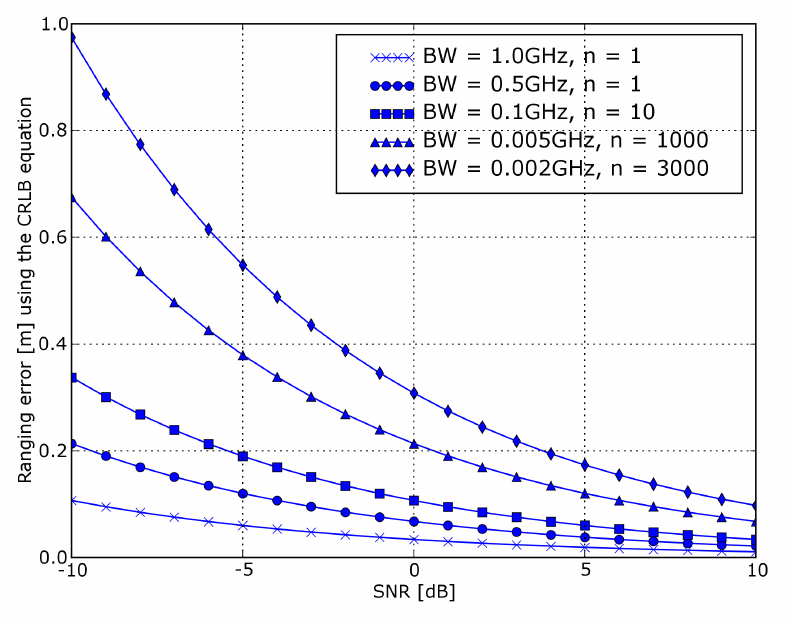
\includegraphics[width=.7\linewidth]{Figures/cramer.png}
    \caption{Нижняя граница диапазона TOF-ошибки}
    \label{fig:cramer}
\end{figure}

Из формулы~\eqref{eq:cramer} видно, что точность TOF-измерения квадратично растёт с увеличением спектральной ширины сигнала, из чего следует эффективность использования сверхширокой полосы. Всвязи с этим, делается вывод о невыгодности использования свободных 433-МГц несущих частот для передачи радиосигнала.
